\def\nodesize{1.0cm}
\tikzstyle{neuron}=[circle, draw=black, minimum size=\nodesize]
\tikzstyle{dots}=[draw=none, scale=2, text height=0.333cm, execute at end node=$\vdots$]

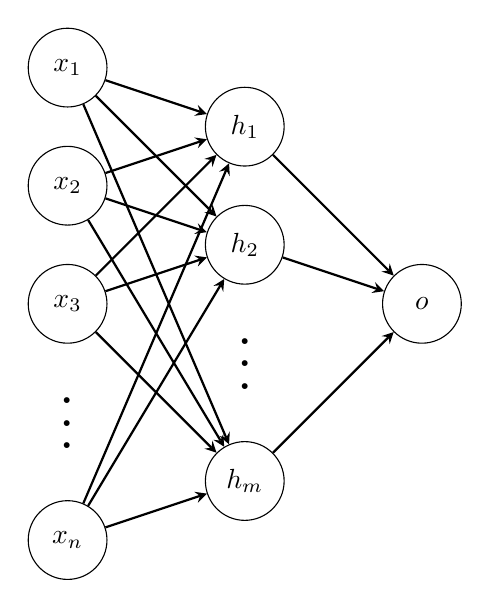
\begin{tikzpicture}[x=1.5cm, y=1.5cm, >=stealth] % >=stealth arrow style
  % input nodes
  \foreach \m [count=\y] in {1,2,3,dots,n} 
  {
    \ifnum\y=4
    \node [\m/.try] at (0,-\y) {};
    \else
    \node [neuron] (input-\m) at (0,-\y) {$x_\m$};
    \fi
  }
  % hidden nodes
  \foreach \m [count=\y] in {1,2,dots,m} 
  {
    \ifnum\y=3
    \node [\m/.try] at (1.5, -\y - 0.5) {};
    \else
    \node [neuron] (hidden-\m) at (1.5, -\y - 0.5) {$h_\m$};
    \fi
  }

  % output node
  \node [neuron] (output) at (3, -3) {$o$};

  % activation function
  % \node [neuron] (activation) at (3.0, -3) {$g$};

  % input-hidden connections
  \foreach \m [count=\y] in {1,2,3,n}
  \foreach \n [count=\y] in {1,2,m}
  % above moves the text higher depending on the orientation of the line
  \draw [thick, ->] (input-\m) -- (hidden-\n) 
  node[above=4pt*abs(3 - \y), pos=0.45, scale=0.9] {};

  % input-hidden connections
  \foreach \m [count=\y] in {1,2,m}
  % above moves the text higher depending on the orientation of the line
  \draw [thick, ->] (hidden-\m) -- (output) 
  node[above=4pt*abs(3 - \y), pos=0.45, scale=0.9] {};
\end{tikzpicture}
